\chapter{Text classification} \label{Text classification}


% The history and different types of classifiers are discussed in this chapter.

\section{A definition of text classification} \label{A definition of text classification}
Text classification is a category of tasks in Natural Language Processing (NLP) which has many real-world applications such as document classification, spam, bot and fraud detection and web search \cite{howard2018,joulin2016}.
A text classification task requires a training set $D = (d_1, \dots , d_n)$ of labelled documents with class $L \in \mathbb{L}$ (e.g. news, politics, sports). Then the task is to determine a \textit{classification model}
\begin{equation}
  f : D \rightarrow \mathbb{L}\qquad f(d) = L
\end{equation}
which assigns the correct class to in domain document $d$.
\cite{hotho}

The labels are assumed to be purely symbolic so that no additional knowledge of their meaning is available, and the data consists of only knowledge extracted from the documents. Thus metadata such as document type, publication date, etc. is not considered available to use.
This ensures that all the methods that will be presented in the coming section are completely general and do not depend on some special-purpose resources.
Given that classification is based on the semantics of documents, which is a subjective notion, the class of a document cannot be deterministically decided.
The phenomenon called \textit{inter-indexer inconsistency} is a result of this undeterministicity which manifests itself when two human experts decide if a document $d_j$ should be classified as $c_i$ and disagree on the matter, which happens surprisingly often \cite{sebastiani2002}.




\section{Text classifiers} \label{Text classifiers}
\subsection{Naive Bayes} \label{Naive Bayes}
The Naive Bayes Classifier is a probabilistic classifier that assumes, like all probabilistic classifiers, that a probabilistic mechanism has generated the words of a document.
It is a simple classifier that estimates the joint probability of a class given a feature vector. It naively assumes that features are independent given class:
\begin{equation}
  P(X|C) = \prod_{i=1}^{n} P(X_{i}|C)
\end{equation}

Where $X = (X_{1},\cdots, X_{n})$ is a feature vector and $C$ is a class.
Even though this assumption is unrealistic, the \textit{naive Bayes} classifier is surprisingly successful in practice \cite{rish}.
Naive Bayes models are very efficient in that they require minimal computational resources even for huge amounts of text and large vocabularies.
There exists a significant problem in this approach, however, named the \textit{never-seen-words} problem which manifests itself when a document containing a word that is not present in the training set is analyzed. The classifier estimates the statistics of a class by counting the occurrences of words in the training set, and a single out-of-vocabulary word will turn the probability of a document belonging to class to 0. This could turn an otherwise clear-cut classed document into something else only due to a random word.
\cite{rigutini2004}

Naive Bayes models have shown good results in various classification tasks and have been used extensively due to their efficiency in training and classification.
A huge setback for the method is its brittleness; to train a robust Naive Bayes Classifier one needs a dataset that covers the problem domain sufficiently, otherwise the model has a high variance. Thus a small dataset performs significantly worse when using a Naive Bayes Classifier than other document classification methods.
\cite{rigutini2004} \cite{lewis1998}

\subsection{Nearest Neighbor Classifier} \label{Nearest Neighbor Classifier}
Nearest neighbor classifiers select documents that are close to the target document instead of building an explicit model. The class of the document can then be inferred from the classes of the neighbouring documents. A classifier that selects the k closest documents is called a \textit{k-nearest neighbor classifier} (kNN).
\cite{hotho}

There are a lot of usable measures for similarity. One example would be to count the number of common words in documents.

When deciding if a document belongs to a class, the document has to be compared to all the document in the training set. Then the k most similar documents are selected and their classes define the probability of whether the document belongs to a certain class or not. The class that has the largest proportion is then assigned to the document. Cross-validation can be used to estimate the optimal number for \textit{k} from additional training data.
\cite{hotho}

Nearest neighbor classifiers are computationally efficient in practice although they require some computation during classification since to determine the nearest neighbors the distance to all samples has to be calculated.
\cite{hotho}
kNNs are more frequently used for unsupervised tasks, such as clustering, rather than supervised tasks.
\cite{rigutini2004}



\subsection{Support Vector Machine} \label{Support Vector Machine}
\begin{figure}[t]
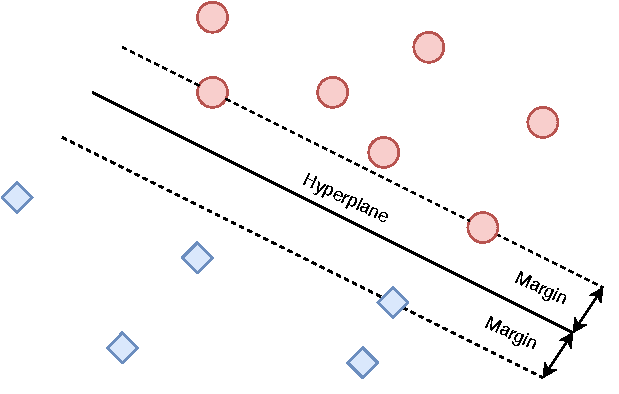
\includegraphics[scale=1]{svm}
\centering
\caption{A hyperplane that separates examples of negative and positive classes with maximal margin}
\label{fig:svm}
\end{figure}
Support vector machines (SVM) are supervised machine learning algorithms that are used for classification and regression analysis.
A single SVM algorithm separates data to two classes by defining a hyperplane that has a maximal distance (margin) to examples of opposing classes (Figure \ref{fig:svm}).
The hyperplane is defined with labeled training data and prediction happens by defining the side in which the example is placed in. If a hyperplane which cuts the data perfectly so that each example is on it's own side is not possible, the algorithm tries to find a division so that as few an example are on the wrong side as possible.
\cite{hotho}
In the case that the given classes can not be separated linearly, SVM transforms ("maps") the input space into a higher dimensional space in which regions can be linearly separated.
\cite{rigutini2004}
Support vector machines can also be used for unsupervised learning, when there is no labeled data, to find a natural grouping by using Support Vector Clustering (SVC)\cite{ben-hur2001}.

SVMs have shown good results in text categorization in the past, are quite computationally efficient and generalize well. Another strength of SVM is that it rarely requires feature selection given that it inherently picks support vectors (individual datapoints) needed for good classification.  \cite{hotho}

\subsection{Decision Trees} \label{Decision Trees}

\begin{figure}[t]
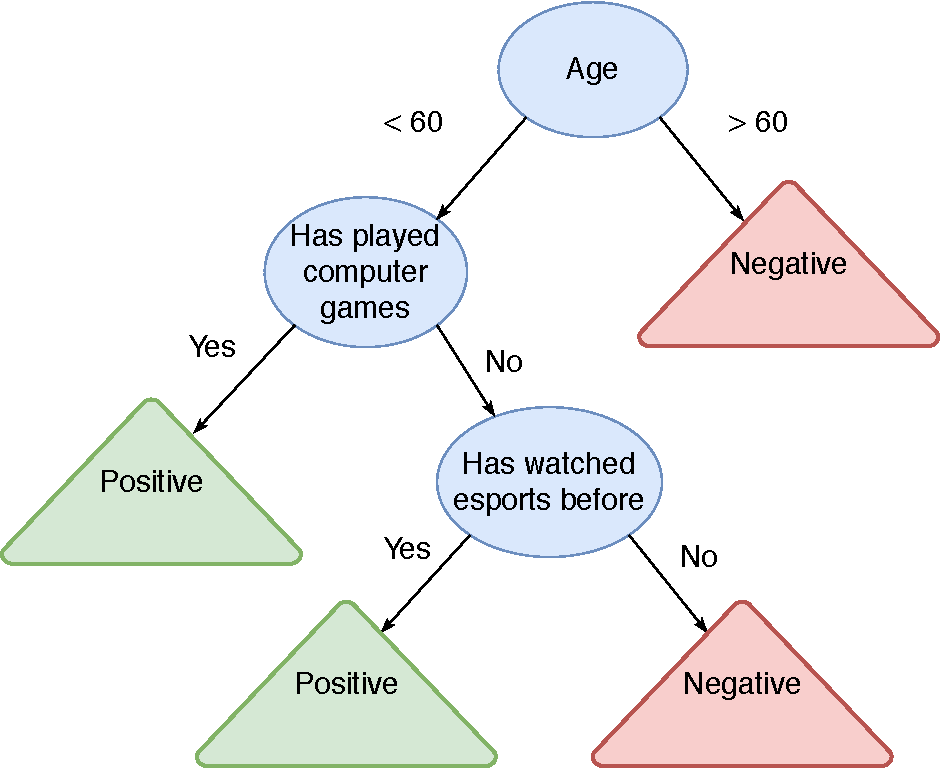
\includegraphics[scale=2]{decision_tree}
\centering
\caption{Example of a simple decision tree which predicts the sentiment of a person regarding esports}
\label{fig:decision_tree}
\end{figure}
Decision trees are classifiers that apply a set of rules sequentially to reach a decision. They can be used for both regression and classification problems and are among the most popular approaches used for text classification.
\cite{hotho} \cite{rokach2005}

Figure \ref{fig:decision_tree} depicts a simple decision tree with three round internal nodes and four triangular leaves. Nodes are labeled with the testable attribute and branches with the attribute's values.

The training process of a text classification decision tree is as follows: Given a training set $M$ with labelled documents, find the word $t_i$ that best predicts the class of the documents. Partition the training set into two subsets, $M^+_i$ and $M^-_i$, with $M^+_i$ containing examples with $t_i$ and $M^-_i$ containing examples without $t_i$. Apply this procedure recursively to $M^+_i$ and $M^-_i$ until all the documents in a subset belong to the same class $L_c$. The generated tree of rules has an assignment to a class as its leaves.
\cite{hotho}


As can be seen from figure \ref{fig:decision_tree}, individual decision trees are quite simple to undestand and to interpret, but are usually not competitive with other supervised learning approaches. They can, however, be dramatically improved by combining multiple trees together to get a consensus prediction with approaches such as \textit{bagging, boosting and random forests} with the cost of losing some interpretability \cite{james2013}.

\subsection{Artificial neural network} \label{Artificial neural network}
\begin{figure}[t]
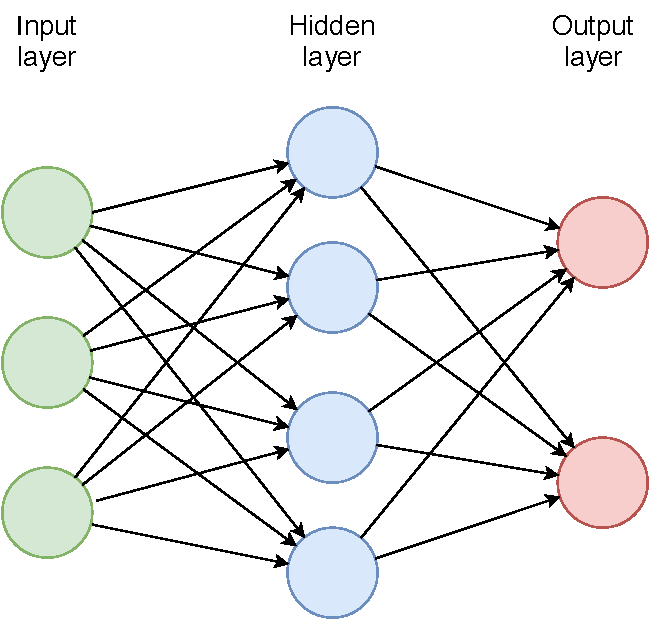
\includegraphics[scale=0.6]{nn}
\centering
\caption{Example of a simple feedforward neural network}
\label{fig:nn}
\end{figure}

A neural network consists of layers of simple processing elements called neurons that are connected to each other.
Each connection has an associated weight that is applied to input.
The first layer is called the input layer after which comes any number of intermediate, or hidden, layers followed by a final output layer.
Neurons are not interconnected within a layer but are only connected to the neurons in adjacent layers.
In a text classifier neural network the prediction of the network can be determined from the values of the final layer's neurons.
For example, a classifier with three different possible classes would have three neurons in the output layer, each corresponding to the probability of a single class \cite{pal1992}.

Neural networks are usually trained using backpropagation which finetunes the parameters of the network by first feeding the network training data, checking the output and if it is misclassified, and then backtracking and updating the weights of the network to eliminate or minimize the error \cite{sebastiani2002}.

The simplest neural network is the single-layer perceptron, introduced by Rosenblatt in 1958 , which consists of a single hidden layer between an input layer and an output layer \cite{rosenblatt1958}.

Since neural networks consist of simple building blocks, layers of neurons or other functions, stacked on top of each other, it allows designing of deep, complex architectures with practically infinite ways of combination.
The depth of a neural network is defined by the number of it's hidden layers.
The latest state-of-the-art neural network models consist of very deep networks with millions of parameters.
